\let\negmedspace\undefined
\let\negthickspace\undefined
\documentclass[journal]{IEEEtran}
\usepackage[a5paper, margin=10mm, onecolumn]{geometry}
\usepackage{tfrupee}

\setlength{\headheight}{1cm}
\setlength{\headsep}{0mm}
\usepackage{gvv-book}
\usepackage{gvv}
\usepackage{cite}
\usepackage{amsmath,amssymb,amsfonts,amsthm}
\usepackage{algorithmic}
\usepackage{graphicx}
\usepackage{textcomp}
\usepackage{xcolor}
\usepackage{txfonts}
\usepackage{listings}
\usepackage{enumitem}
\usepackage{mathtools}
\usepackage{gensymb}
\usepackage{comment}
\usepackage[breaklinks=true]{hyperref}
\usepackage{tkz-euclide}
\def\inputGnumericTable{}
\usepackage[latin1]{inputenc}
\usepackage{color}
\usepackage{array}
\usepackage{longtable}
\usepackage{calc}
\usepackage{multirow}
\usepackage{hhline}
\usepackage{ifthen}
\usepackage{lscape}
\usepackage{booktabs}
\usepackage{tikz}
\usetikzlibrary{arrows.meta,angles,quotes}

\begin{document}

\bibliographystyle{IEEEtran}
\vspace{3cm}

\section*{\large\textbf{Problem 7.2.5}}
\vspace{0.5cm}

Check whether the point \( \vec{P} = \myvec{-2 \\ 4} \) lies on a circle of radius 6 centered at  
\( \vec{C} = \myvec{3 \\ 5} \).

\section*{\large\textbf{Matrix Form}}
\vspace{0.5cm}

The general equation of a circle with center \( \vec{C} \) and radius \( r \) is:

\[
\|\vec{x} - \vec{C}\|^2 = r^2
\]

Substituting \( \vec{C} = \myvec{3 \\ 5} \), \( r = 6 \):

\[
\|\vec{x} - \myvec{3 \\ 5}\|^2 = 36
\]

Expanding the norm:

\[
(\vec{x} - \myvec{3 \\ 5})^T (\vec{x} - \myvec{3 \\ 5}) = 36
\]

\section*{\large\textbf{Substitution}}
\vspace{0.5cm}

Let \( \vec{x} = \vec{P} = \myvec{-2 \\ 4} \). Then:

\[
(\myvec{-2 \\ 4} - \myvec{3 \\ 5})^T (\myvec{-2 \\ 4} - \myvec{3 \\ 5})
= \myvec{-5 \\ -1}^T \myvec{-5 \\ -1}
= (-5)^2 + (-1)^2 = 25 + 1 = 26
\]

\section*{\large\textbf{Comparison}}
\vspace{0.5cm}

\[
\text{LHS} = 26, \quad \text{RHS} = 36
\Rightarrow 26 \ne 36
\]

\section*{\large\textbf{Conclusion}}
\vspace{0.5cm}

The point \( \vec{P} = \myvec{-2 \\ 4} \) does not satisfy the equation of the circle.  
Hence,  
\[
\boxed{\vec{P} \text{ does not lie on the circle}}
\]


\begin{figure}[h!t]
\centering
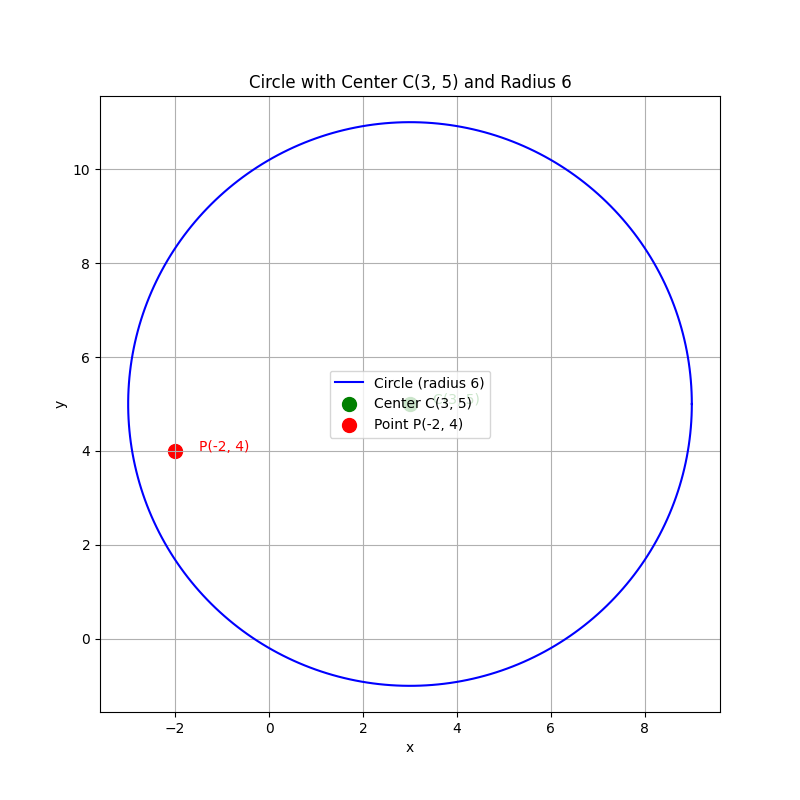
\includegraphics[width=0.9\linewidth]{Figs/Fig1.png}
\caption{Circle and the point}
\end{figure}

\end{document}












